\documentclass[a4,10pt]{aleph-notas}

% -- Paquetes adicionales
\usepackage{enumitem}
\usepackage{aleph-comandos}
\usepackage{quantikz}

% -- Datos
\institucion{Proyecto Alephsub0}
\asignatura{Computación Cuántica}
\tema{Codificación superdensa}
\autor{Andrés Merino}
\fecha{Julio 2026}

\fuente{montserrat}
\logouno[4.5cm]{Logos/LogoAlephsub0-02}
\definecolor{colordef}{cmyk}{0.81,0.62,0.00,0.22}

% -- Comandos adicionales
\newtheorem*{prob}{Problema}
    \tcolorboxenvironment{prob}{%
        color=colordef,recuadrost,colback=colordef!7,drop fuzzy shadow
    }

\begin{document}


\encabezado

La codificación superdensa es un circuito que logra transmitir dos bits de información clásica utilizando un solo cúbit, aprovechando el entrelazamiento cuántico.

La idea es:
\begin{itemize}
    \item Se entrelazan dos cúbits y se distribuyen el primero para el emisor (Alice) y el segundo para el receptor (Bob). Esto debe ser realizado como paso previo a la comunicación.
    \item Alice desea enviar dos bits de información clásica a Bob. Para ello, aplica una transformación a su cúbit dependiendo de los bits $(a,b)$ que desea enviar.
    \item Luego, Alice envía su cúbit a Bob.
    \item Bob recibe el cúbit de Alice y, junto con su propio cúbit, realiza una medición que le permite recuperar los dos bits de información que Alice quería enviar.
\end{itemize}

El circuito de codificación superdensa es:
\begin{center}
    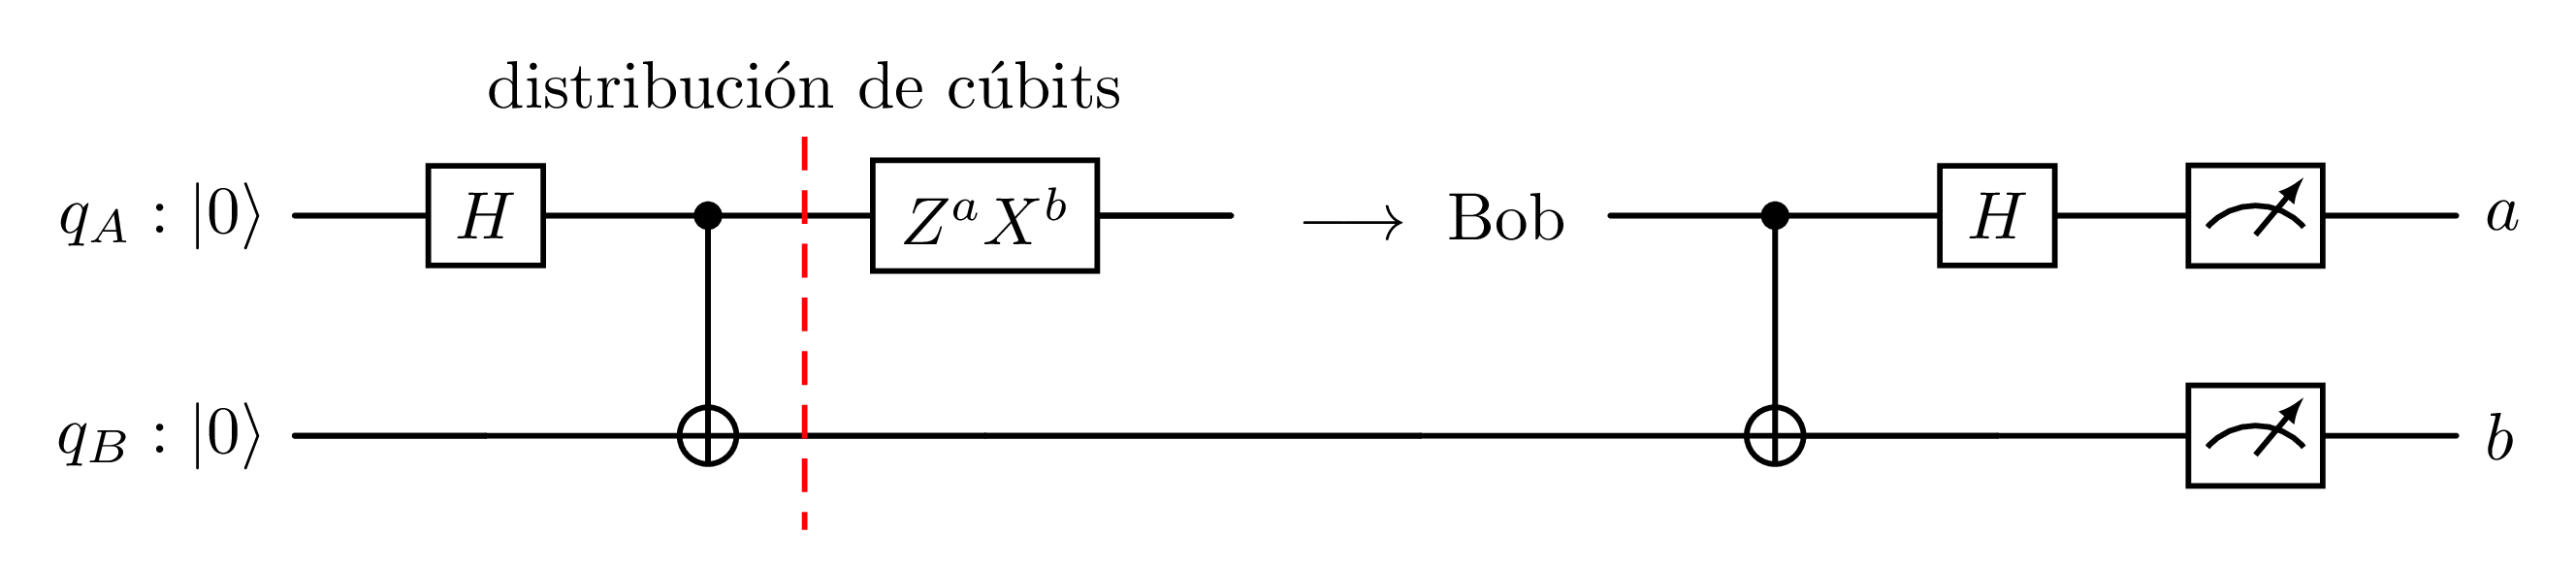
\includegraphics[width=0.8\textwidth]{imagen.png}
\end{center}

\begin{prob}
    Realizar la derivación matemática de la codificación superdensa.
\end{prob}


\begin{proof}
    Sean \(q_A\) y \(q_B\) los cúbits asociados con Alice y Bob,
    respectivamente. Inicialmente, ambos cúbits se encuentran en el estado
    \[
        \ket{q_Aq_B}=\ket{00}.
    \]

    Consideremos los siguientes pasos del circuito:
    \begin{center}
        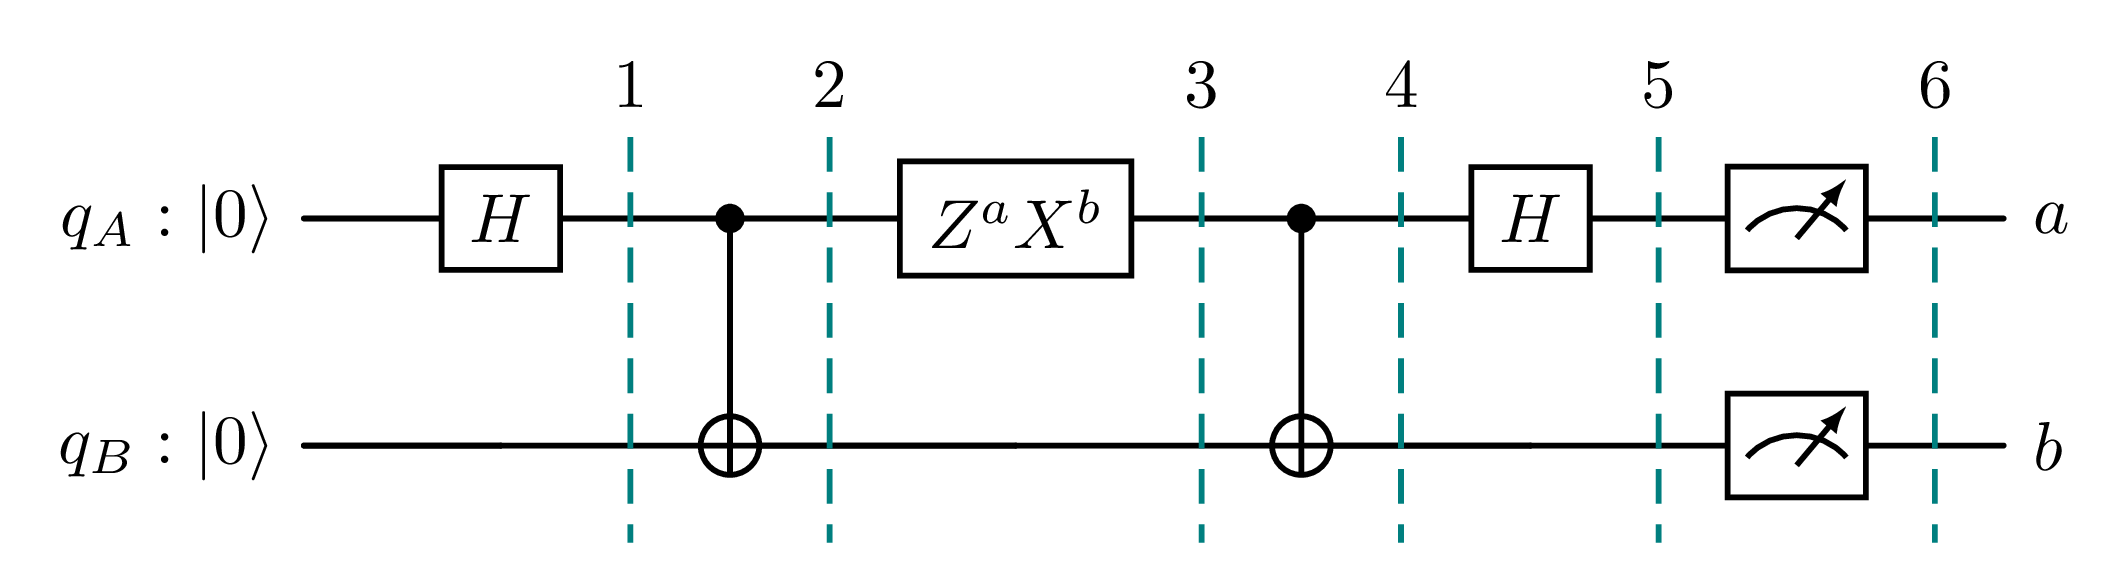
\includegraphics[width=0.8\textwidth]{imagen2.png}
    \end{center}

    \begin{itemize}
        \item \textbf{Paso 1.} Se aplica la compuerta Hadamard al primer cúbit:
        \[
            (H\otimes I)\ket{00}
            =H\ket{0}\otimes\ket{0}
            =\frac{1}{\sqrt{2}}
            \left(\ket{00}+\ket{10}\right).
        \]

        \item \textbf{Paso 2.} Se aplica la compuerta CNOT, utilizando el primer
        cúbit como control y el segundo como objetivo:
        \[
            \operatorname{CNOT}
            \frac{1}{\sqrt{2}}
            \left(\ket{00}+\ket{10}\right)
            =
            \frac{1}{\sqrt{2}}
            \left(\ket{00}+\ket{11}\right).
        \]
        Se obtiene así el estado de Bell
        \[
            \ket{\Phi^+}
            =
            \frac{1}{\sqrt{2}}
            \left(\ket{00}+\ket{11}\right).
        \]
        El primer cúbit se entrega a Alice y el segundo a Bob.

        \item \textbf{Paso 3.} Para codificar los bits clásicos \(a,b\in\{0,1\}\),
        Alice aplica la transformación
        \[
            Z^aX^b
        \]
        sobre su cúbit. Por tanto, el estado conjunto se transforma en
        \[
            \ket{\psi_{ab}}
            =
            (Z^aX^b\otimes I)\ket{\Phi^+}.
        \]
        Los cuatro posibles estados son:
        \begin{align*}
            \ket{\psi_{00}}
            &=
            \frac{1}{\sqrt{2}}
            \left(\ket{00}+\ket{11}\right),\\
            \ket{\psi_{01}}
            &=
            \frac{1}{\sqrt{2}}
            \left(\ket{01}+\ket{10}\right),\\
            \ket{\psi_{10}}
            &=
            \frac{1}{\sqrt{2}}
            \left(\ket{00}-\ket{11}\right),\\
            \ket{\psi_{11}}
            &=
            \frac{1}{\sqrt{2}}
            \left(\ket{01}-\ket{10}\right).
        \end{align*}
        Después de realizar la codificación, Alice envía su cúbit a Bob.

        \item \textbf{Paso 4.} Bob aplica nuevamente una compuerta CNOT, con el
        primer cúbit como control y el segundo como objetivo:
        \begin{align*}
            \operatorname{CNOT}\ket{\psi_{00}}
            &=
            \frac{1}{\sqrt{2}}
            \left(\ket{00}+\ket{10}\right),\\
            \operatorname{CNOT}\ket{\psi_{01}}
            &=
            \frac{1}{\sqrt{2}}
            \left(\ket{01}+\ket{11}\right),\\
            \operatorname{CNOT}\ket{\psi_{10}}
            &=
            \frac{1}{\sqrt{2}}
            \left(\ket{00}-\ket{10}\right),\\
            \operatorname{CNOT}\ket{\psi_{11}}
            &=
            \frac{1}{\sqrt{2}}
            \left(\ket{01}-\ket{11}\right).
        \end{align*}
        Estas expresiones pueden factorizarse como
        \begin{align*}
            \operatorname{CNOT}\ket{\psi_{00}}
            &=\ket{+}\ket{0},\\
            \operatorname{CNOT}\ket{\psi_{01}}
            &=\ket{+}\ket{1},\\
            \operatorname{CNOT}\ket{\psi_{10}}
            &=\ket{-}\ket{0},\\
            \operatorname{CNOT}\ket{\psi_{11}}
            &=\ket{-}\ket{1},
        \end{align*}
        donde
        \[
            \ket{+}
            =
            \frac{\ket{0}+\ket{1}}{\sqrt{2}},
            \qquad
            \ket{-}
            =
            \frac{\ket{0}-\ket{1}}{\sqrt{2}}.
        \]

        \item \textbf{Paso 5.} Bob aplica la compuerta Hadamard al primer cúbit.
        Puesto que
        \[
            H\ket{+}=\ket{0},
            \qquad
            H\ket{-}=\ket{1},
        \]
        se obtiene
        \begin{align*}
            (H\otimes I)\operatorname{CNOT}\ket{\psi_{00}}
            &=\ket{00},\\
            (H\otimes I)\operatorname{CNOT}\ket{\psi_{01}}
            &=\ket{01},\\
            (H\otimes I)\operatorname{CNOT}\ket{\psi_{10}}
            &=\ket{10},\\
            (H\otimes I)\operatorname{CNOT}\ket{\psi_{11}}
            &=\ket{11}.
        \end{align*}

        \item \textbf{Paso 6.} Finalmente, Bob mide ambos cúbits en la base computacional y obtiene el resultado \(\ket{ab}\). De esta manera, recupera exactamente los dos bits clásicos enviados por Alice.
    \end{itemize}

    Por tanto, mediante el envío de un solo cúbit y el uso previo de un par
    entrelazado, Alice puede transmitir dos bits clásicos a Bob.
\end{proof}




\end{document}